\section{On Maps}

\newcommand{\mywidth}{0.875\textwidth} 

\begin{tcbraster}[
    raster columns = 3,
    raster equal height,
    colback = white,
    raster equal skip = 0mm,
]
\begin{tcolorbox}[colframe=white]
    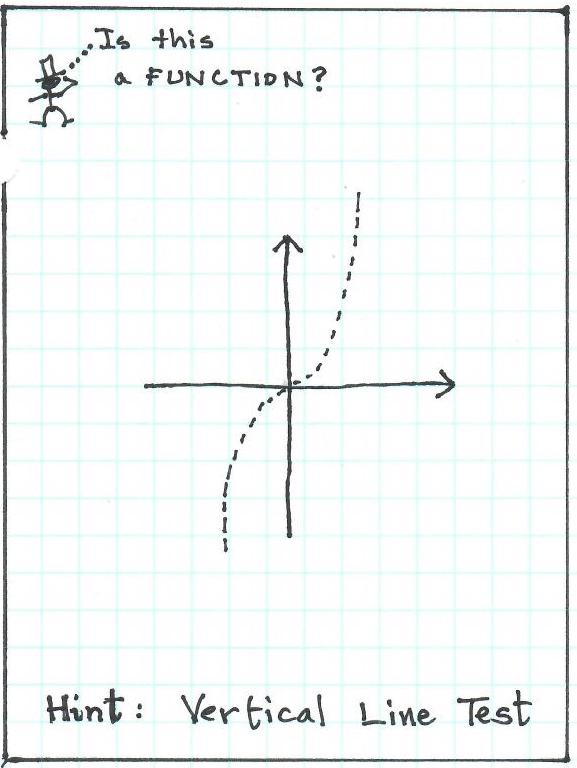
\includegraphics[width=\mywidth]{on-maps-1.jpg}
\end{tcolorbox}
\begin{tcolorbox}[colframe=white]
    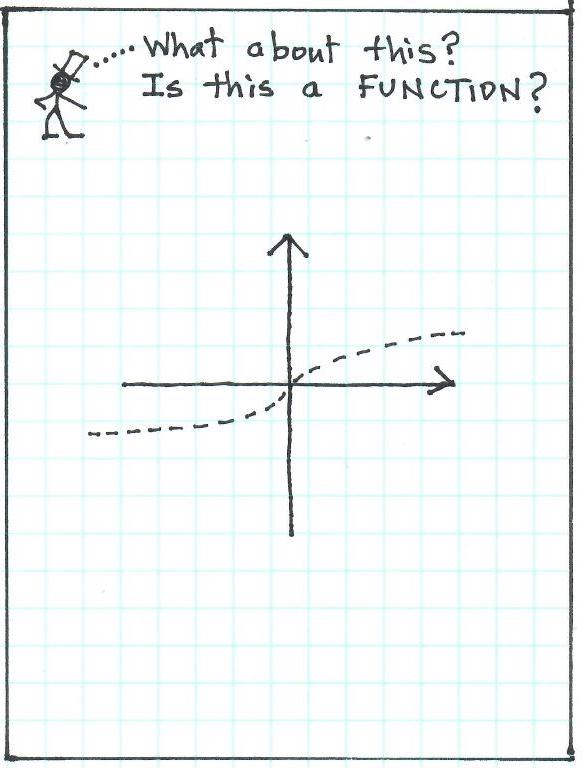
\includegraphics[width=\mywidth]{on-maps-2.jpg}
\end{tcolorbox}
\begin{tcolorbox}[colframe=white]
    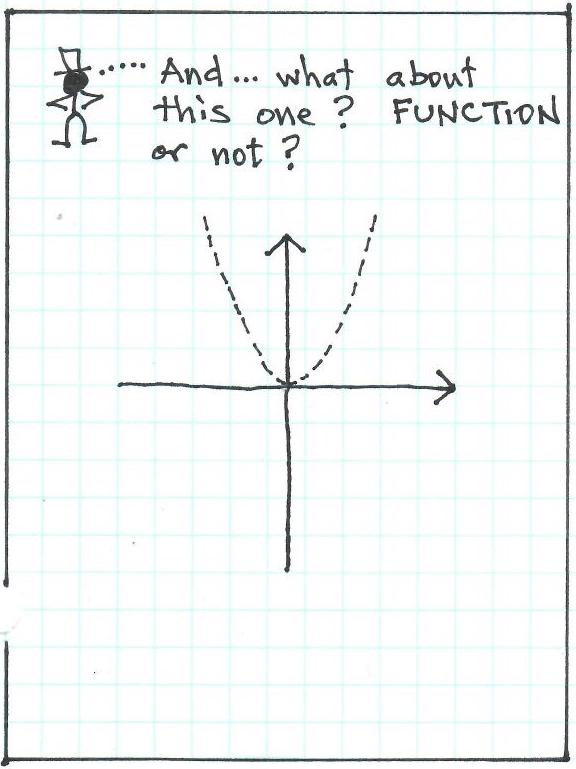
\includegraphics[width=\mywidth]{on-maps-3.jpg}
\end{tcolorbox}
%
\begin{tcolorbox}[colframe=white]
    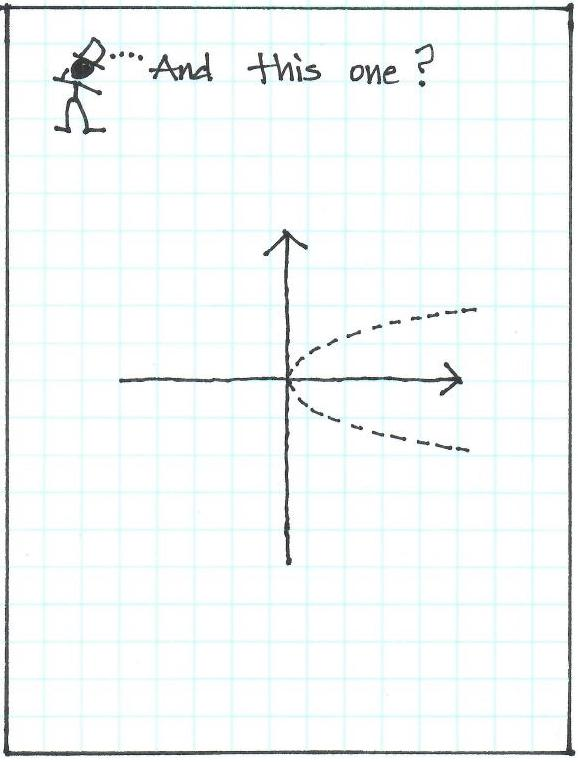
\includegraphics[width=\mywidth]{on-maps-4.jpg}
\end{tcolorbox}
\begin{tcolorbox}[colframe=white]
    
\includegraphics[width=\mywidth]{on-maps-5.jpg}
\end{tcolorbox}
\begin{tcolorbox}[colframe=white]
    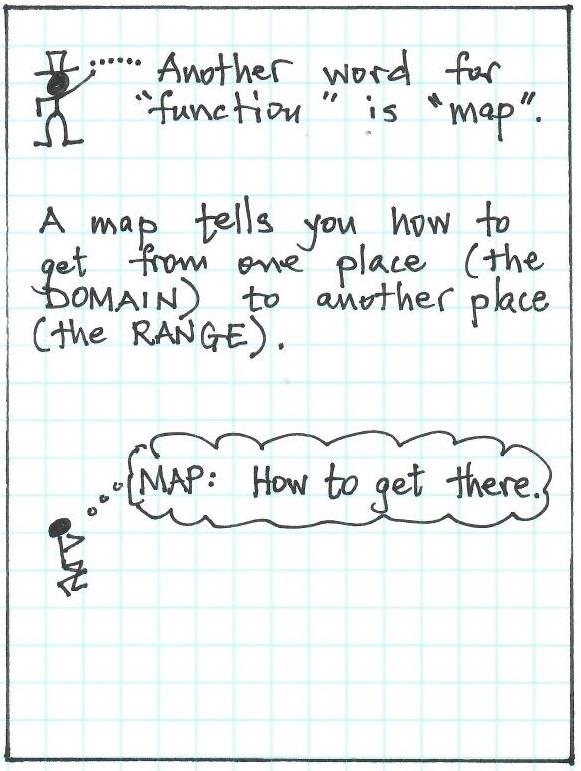
\includegraphics[width=\mywidth]{on-maps-6.jpg}
\end{tcolorbox}
\end{tcbraster}


\begin{tcbraster}[
    raster columns = 3,
    raster equal height,
    colback = white,
    raster equal skip = 0mm,
]
\begin{tcolorbox}[colframe=white]
    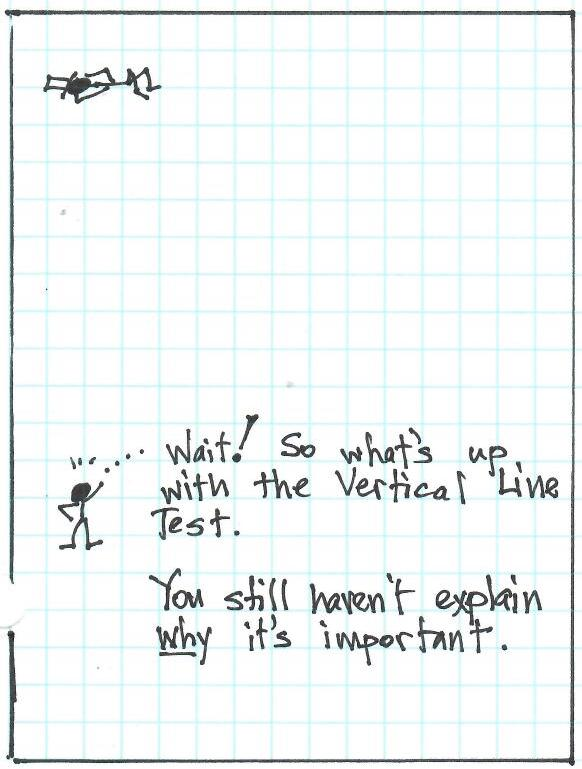
\includegraphics[width=\mywidth]{on-maps-7.jpg}
\end{tcolorbox}
\begin{tcolorbox}[colframe=white]
    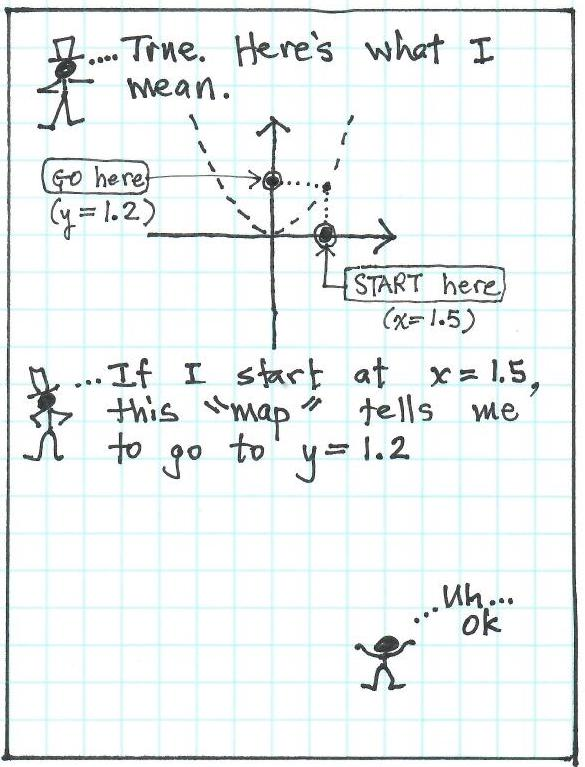
\includegraphics[width=\mywidth]{on-maps-8.jpg}
\end{tcolorbox}
\begin{tcolorbox}[colframe=white]
    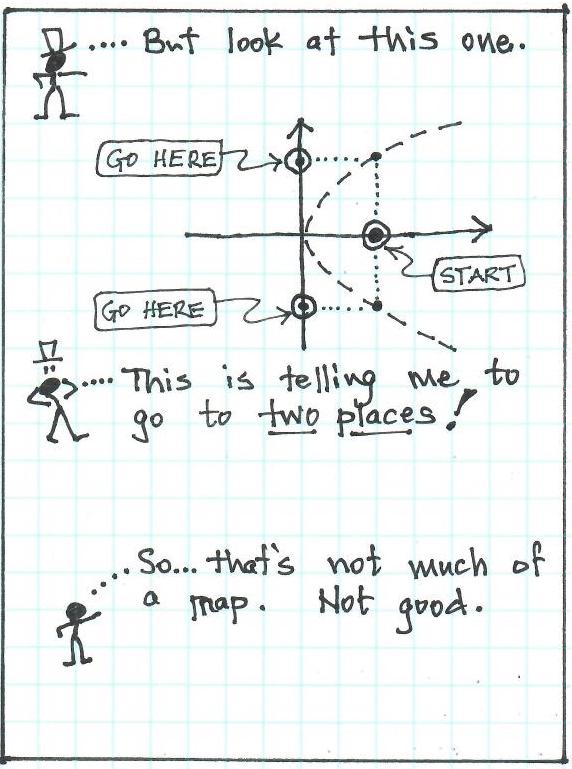
\includegraphics[width=\mywidth]{on-maps-9.jpg}
\end{tcolorbox}
%
\begin{tcolorbox}[colframe=white]
    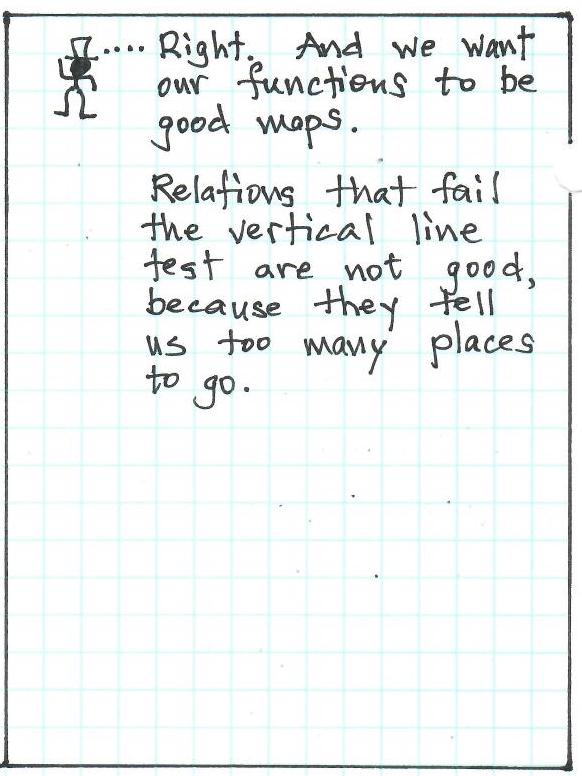
\includegraphics[width=\mywidth]{on-maps-10.jpg}
\end{tcolorbox}
\begin{tcolorbox}[colframe=white]
    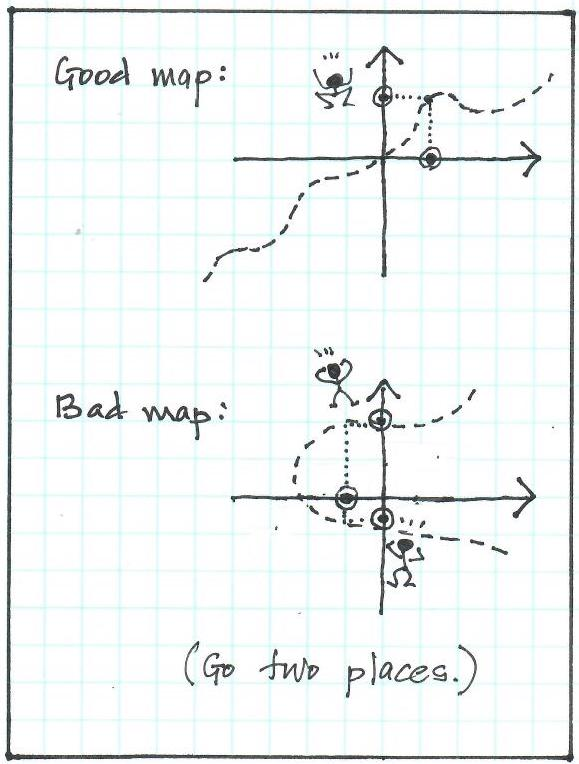
\includegraphics[width=\mywidth]{on-maps-11.jpg}
\end{tcolorbox}
\begin{tcolorbox}[colframe=white]
    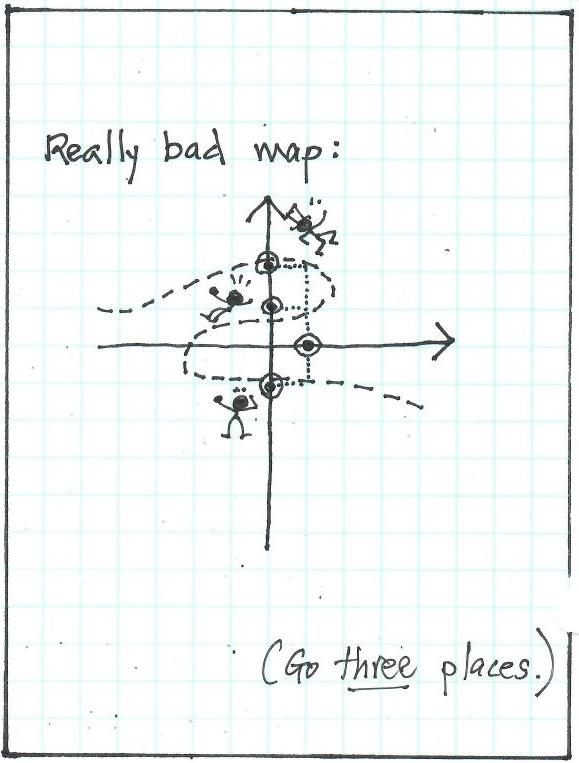
\includegraphics[width=\mywidth]{on-maps-12.jpg}
\end{tcolorbox}
\end{tcbraster}

\begin{myConcept}{To read the map\dots}
    \begin{itemize}[nosep]
        \item Start on the $x$-axis.
        \item Draw a \gap{vertical} \gap{arrow} up to the graph.
        \item Then draw a \gap{horizontal} \gap{arrow} over to the $y$-axis.
        \item This takes you from $x\mapsto y$.
    \end{itemize}
\end{myConcept}